\subsection{3D Rectification}


\begin{figure}[h!]
  \centering
  \resizebox{0.45\textwidth}{!}{
  \resizebox{0.8\textwidth}{!}{\minipage{0.3\textwidth}
      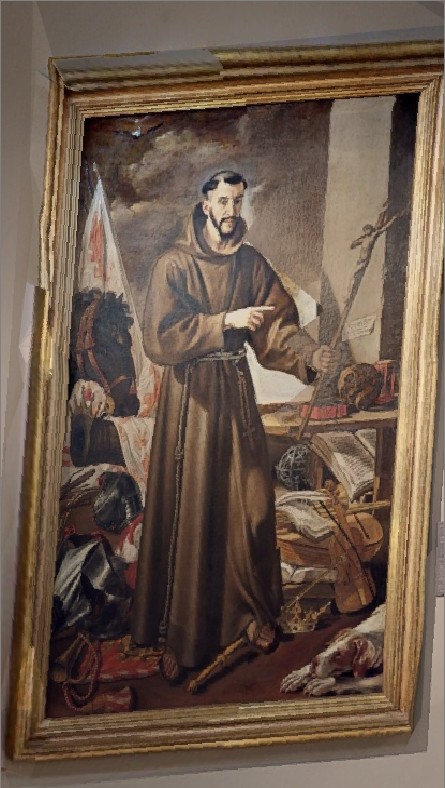
\includegraphics[width=\linewidth]{pictures/painting_detection/3d_rectification_original.PNG}
      \caption*{Original 3D model painting}\label{fig:rectification_original}
    \endminipage\hfill}
    \resizebox{0.8\textwidth}{!}{\minipage{0.3\textwidth}
      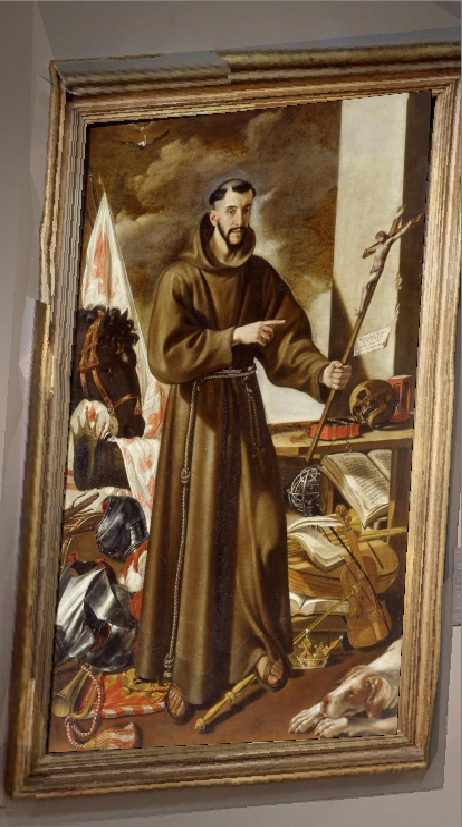
\includegraphics[width=\linewidth]{pictures/painting_detection/3d_rectification_warped.PNG}
      \caption*{Replaced painting}\label{fig:rectification_warped}
    \endminipage\hfill}}
    \caption{Painting rectification from the 3D view}\label{fig:3d-warping}
\end{figure}


The 3D Rectification is the last optional task that has been done. The scope was to replace the painting that was present in a 3D model with the same painting but with an higher resolution. Have been taken some screenshot of the 3D model with an off-line approach, then were extracted all the ROI that were present in the acquired image and each painting of the model was confronted with all the painting in our database. The painting identified was first warped with an homography trasformation in order to be in the same prospective of the painting in the screenshot and then was replaced with the previous one; in case of mismatch nothing was done. One of the results that has been achieved is showed in the fig.~\ref{fig:3d-warping}.
